\documentclass{frontiersSCNS} % for Science articles

\usepackage[english]{babel}

%\setcitestyle{square}
\usepackage{url,lineno}
\linenumbers

\usepackage{datetime}
\usepackage{fmtcount}
\usepackage{etoolbox}

\usepackage{amsmath} 
\usepackage{mathptmx}

\usepackage{array}
\usepackage{graphicx}
%\usepackage{caption}
%\usepackage{subcaption}
\graphicspath{{figs/}}

\usepackage{color, soul}
\usepackage{url}
\usepackage{multirow}
\usepackage{array}
\usepackage{fixltx2e}
\usepackage{textcomp}

\newcommand{\eg}{{\textit{e.g.~}}}
\newcommand{\etal}{{\textit{et al.~}}}
\newcommand{\ie}{{\textit{i.e.~}}}
\newcommand{\etc}{{\textit{etc.~}}}
\newcommand{\vs}{{\textit{vs.~}}}

\hyphenation{com-mon-ly}
\hyphenation{an-thro-po-mor-phism}
\hyphenation{an-thro-po-mor-phic}

% Leave a blank line between paragraphs in stead of using \\

\copyrightyear{}
\pubyear{}

\def\journal{Cognitive Science}%%% write here for which journal %%%
\def\DOI{}
\def\articleType{Hypothesis and Theory}
\def\keyFont{\fontsize{8}{11}\helveticabold }
\def\firstAuthorLast{Fink {et~al.}} %use et al only if is more than 1 author
\def\Authors{Julia Fink\,$^{1*}$, S\'{e}verin Lemaignan$^{1}$, Claire Braboszcz$^{2}$ and Pierre Dillenbourg$^{1}$}
\def\Address{$^{1}$Computer-Human Interaction in Learning and Instruction (CHILI) \\ Ecole Polytechnique F\'{e}d\'{e}rale de Lausanne (EPFL) \\ CH-1015 Lausanne, Switzerland \\
\vspace{0.25cm}
$^{2}$Laboratory for Neurology and Imaging of Cognition (LabNIC) \\
Universit\'{e} de Gen\`{e}ve \\ CH-1211 Gen\`{e}ve, Switzerland 
}
\def\corrAuthor{Julia Fink \vspace{1mm}}
\def\corrAddress{EPFL - CHILI, RLC D1 740, Station 20, CH-1015 Lausanne, Switzerland}
\def\corrEmail{julia.fink@epfl.ch}


\begin{document}
\onecolumn
\firstpage{1}

\title[Dynamics of Anthropomorphism]{Dynamics of Anthropomorphism in Human-Robot Interaction}
\author[\firstAuthorLast ]{\Authors}
\address{}
\correspondance{}
\extraAuth{}
\topic{The Uncanny Valley Hypothesis and Beyond}% If your article is part of a Research Topic, please indicate here which.


\maketitle


\begin{abstract}

%As a primary goal, the abstract should render the general significance and conceptual advance of the work clearly accessible to a broad readership. References should not be cited in the abstract.

\textit{Anthropomorphism} -- people's tendency to perceive human-like characteristics in non-human agents -- is a commonly observed phenomenon in Human-Robot Interaction (HRI). Though having been extensively studied, anthropomorphism is still not very well understood. Often, anthropomorphism is analyzed from the sole perspective of the human-like (anthropomorphic) design of a robot. 
%The question in focus is to what extent different types of anthropomorphic robot designs evoke affinity or uncanny feelings in the human user.
%In this regard, the \textit{Uncanny Valley} hypothesis suggests that an anthropomorphic design can evoke both positive and negative feelings in human users, determined by the degree of human-likeness. 
We believe that we need to go beyond this, in order to gain a better awareness about the phenomenon as a whole. To this end, we make three suggestions toward extending our understanding of anthropomorphism in HRI.
First, we suggest to comprehend anthropomorphism as a human-centered social phenomenon that arises in an interaction between a human and a robot in a specific context (partly determined by the purpose of the robot). Consequently, we propose that \textbf{multiple factors} need to be considered: the characteristics of the robot, of the human, and of the context. This holds implications for how anthropomorphism is studied and measured.
%Real physical interaction is required.
By applying a cognitive perspective, we further suggest that anthropomorphism is \textbf{multi-layered}, not being either \textit{there} or \textit{not there} but that there exist lower and higher levels of it, depending on the \textit{cognitive depth} that the attribution of a human-like characteristic to the robot implies, as well as on the specific mental model on which it is based.
Finally, we hypothesize that anthropomorphism is \textbf{dynamic}. In other words, it evolves over time, with growing real or imagined interaction experience and familiarization of the human user with the robot.
We formalize our ideas in a conceptual model that we call the \textit{Dynamics of Anthropomorphism}. Our hypotheses are based on results from our own empirical interaction studies, and informed on a review of related work in psychology, cognitive science and neuroscience as well as on previous research in HCI and HRI.
%As a consequence of our hypotheses, we discuss the methods and measurement tools to study anthropomorphism and propose going toward long-term interaction studies to verify our conceptual model.


\tiny
\keyFont{ \section{Keywords:} Anthropomorphism, Design, Dynamics, Human-Robot 
Interaction, Mental Models, Robot Acceptability, Social Robotics} 
\end{abstract}

%%%%%%%%%%%%%%%%%%%%%%%%%%%%%%%%%%%%%%%%%%%%%%%%%%%%%%%%%%%%%
%
%
%
%		INTRODUCTION
%
%
%
%%%%%%%%%%%%%%%%%%%%%%%%%%%%%%%%%%%%%%%%%%%%%%%%%%%%%%%%%%%%%


\section{Introduction}
\label{sec:introduction}

Anthropomorphism can be seen as a special type of
social response that people commonly show when interacting with 
robots. The phenomenon has been observed related to various types of technology, virtual agents, daily life objects, animals, and even simple geometric moving shapes. It seems that people have an almost natural tendency to \textit{``see human in the nonhuman''} -- and ascribe human-like characteristics to basically anything that acts or is believed to act with apparent independence \citep{epley_seeing_2007}. We focus here on anthropomorphism related to robots. In HRI it is commonly described that users tend to perceive and treat their robot as having some human-like characteristics, and hence attribute, for instance, emotional states, motivations, or intentions to it. Some Roomba (vacuum cleaning robot) owners even ascribe personality and gender to their robot and choose a name for it \citep{forlizzi_service_2006,forlizzi_how_2007,krumm_my_2007,sung_domestic_2010}.
To what extent people anthropomorphize a robot has so far mostly been studied from the sole perspective of the design of a robot. In short, the general assumption is that the more human-like a robot looks like and behaves, the more people will anthropomorphize it.
Not necessarily related to anthropomorphism but focusing on the uncanny aspect, Mori's \textit{Uncanny Valley} hypothesis suggests that the relation between the robot's degree of anthropomorphic form and people's feelings toward it is non-linear \citep{mori_uncanny_1970,mori_uncanny_2012}.
Somewhat similar to this non-linear relation between a robot's design and people's feeling toward it, we suspect that also people's tendency to anthropomorphize a robot is of dynamic nature. Furthermore, we hypothesize that the robot's design (its degree of anthropomorphic form) is not the only factor that plays a role in how much the robot is anthropomorphized by a user.

So far, the idea of multiple factors, as well as the dynamic nature of anthropomorphism have been mostly disregarded. There exists no research that investigated how anthropomorphism evolves over longer periods of time based on repeated physical interactions between the human and the robot. This is, however, a relevant aspect to investigate. Long-term interaction studies found that people's perception of a robot, their attitude toward it, how they use it, and how they experience it changes over time \citep{kanda_interactive_2004,karapanos_user_2009,sung_domestic_2010}. It is described that besides \textit{novelty effects} also the user's increasing \textit{familiarity} with the robot over time play a role and hence, we assume that this also impacts how much the robot will be anthropomorphized. We will shed light on this aspect by taking a (developmental / social) psychology and cognitive science perspective because these fields provide interesting explanations for people's tendency to anthropomorphize and we believe this can offer relevant extensions to our understanding of the phenomenon in HRI. Our general aim is to deepen our understanding of anthropomorphism, in order to advance research on this topic. We make three suggestions that can be addressed in future empirical research. Namely, we propose that anthropomorphism is based on multiple factors, that it is multi-layered, and that it is of dynamic nature.

%This is mostly theoretical material, gathered by reviewing diverse literature, reflecting upon it and integrating it. Anthropomorphism has first not been our main research topic, however, what led us to investigate the phenomenon in more detail, were surprising findings from our own HRI studies in which we observed anthropomorphism as an emerging phenomenon.
%We illustrate some of our empirical data and give concrete examples, so to stimulate the discussion about the current understanding of anthropomorphism, and guide the reader towards our ideas. One suggestion is, for instance, to measure anthropomorphism as being a characteristic of an interaction and not only of a user's perception of a robot.  

%The proposed dynamics of anthropomorphism also implicate that we need to find new methods and tools to measure anthropomorphism, and we would like to take an initial step toward this by introducing a so-called \textit{anthropomorphism index}. 


%
%Another reason may be that most of the research that examines the \textit{Uncanny Valley} is conducted in absence of real interaction but uses photos or videos of different robots instead. Furthermore, to measure anthropomorphism, mostly rating scales and questionnaires are applied. Based on our understanding of anthropomorphism we see a limitation in this, which we would like to discuss later. 

%\footnote{To facilitate things, we use the terms \textit{`non-human 
%agent'}, \textit{`system'} and \textit{`robot'}, as well as 
%\textit{`artifact'} more or less interchangeably throughout this 
%article. Similarly, the terms \textit{`users'}, 
%\textit{`observers'}, \textit{`people'} and \textit{`humans'} are 
%used as synonyms.} 
%
%

%
%This idea is supported by a child-robot interaction study that we carried out with twenty-six 4-5 year old children.\footnote{A publication about this study is in work.} In a playful task, each two children were collaborating with our robotic box ``Ranger'' \citep{fink_which_2014} to assemble a domino. From time to time, the robot showed some unexpected behavior and we assessed to what extent children anthropomorphized the robot, \textit{e.g.} by ascribing intention or emotional states to robot.
%We found that children commonly attributed only some types of human-like characteristics, such as perceptual skills (which are not uniquely human), feeling, and moral standing. Also, children perceived the robot as a social entity and agreed it could be their friend. However, the majority of children did not ascribe intention to the robot ...

%So far in human-robot interaction (HRI), the study of anthropomorphism has mostly centered on the anthropomorphic design of a robot and its influence on people's perception of the robot. For instance, a prominent question is how more and less anthropomorphic robots (\textit{e.g.}, humanoid robot \textit{vs.} mechanic robot) are perceived in terms of human-likeness and to what extent the different designs evoke feelings of closeness / affinity or reluctance / revulsion. The so-called \textit{Uncanny Valley} hypothesis \citep{mori_uncanny_1970} states a non-linear relationship between these two variables, which has provoked a lot of research, which produced partly controversial findings, however.

%Not focusing on the uncanny aspect of a human-like robot design, a general question is whether people perceive and treat a human-like robot more readily as if it was a human. This is one of the major research topics in social robotics.

\subsection{What is Anthropomorphism?}
\label{sec:definitions}

Literature on anthropomorphism is diverse and there exist different and partly conflicting definitions (across and within disciplines). As a result of this, there are also different understandings of what exactly (which phenomenon) `anthropomorphism' describes.
%This may be due to the fact that anthropomorphism is studied in a variety of different domains that each integrate their own understanding and use the same terms to refer to different phenomena.
The problem is that despite the lack of a commonly accepted definition, the terms `anthropomorphism' and `anthropomorphic' are often used as if their meanings were clear and agreed upon \citep{persson_anthropomorphism_2000}. Especially in a multi-disciplinary field like HRI this can lead to a conflict. Thus, we have to be clear and specific about what we mean when we talk about anthropomorphism.

We propose to use the term `anthropomorphism' to refer to a specific \textit{human-centered social phenomenon} but to \textit{not} use the same term to refer to the amount of human-likeness in the \textit{design} of a robot (for latter one, we propose to use alternative formulations, such as `anthropomorphic design' or `human-like form'.) We believe that this differentiation is necessary and important. The point that we want to make is, that anthropomorphism arises in an interaction and as such, a robot does not \textit{``contain anthropomorphism''} or have a specific level of anthropomorphism in itself, but that it only gives rise to the process of being anthropomorphized by a given user. The ambiguity of terms has been previously discussed \citep{persson_anthropomorphism_2000,duffy_anthropomorphism_2002}.\footnote{Several attempts have been made to clarify what exactly anthropomorphism is. \cite{epley_when_2008} approached the issue from a psychological point of view give several examples of what anthropomorphism is \textit{not}. The reader may refer to the original work for more details.}  

More specifically, we use the term `anthropomorphism' to describe a social phenomenon that arises in a real or imagined interaction between a human and a robot in a given context (see Figure~\ref{fig:multiple-factors}). The active player (the one who anthropomorphizes) is the human, and therefore, the phenomenon itself is human-centered. (Explanations of anthropomorphism can apply both a human-centered and an artifact-centered perspective, depending on the direction of causality which is studied: Is the human himself motivated to anthropomorphize the robot or is the robot, which leads the human to anthropomorphize it?) In our understanding, anthropomorphism includes both people's tendency to \textit{perceive / image} human-like characteristics in a robot, as well as the action of verbally \textit{ascribing / attributing} these characteristics to the robot and \textit{reacting / behaving / treating} the robot alike. Consequently, we believe that anthropomorphism can not only be assessed as a variable of a person's perception of the robot but also be observed in how he/she interacts with the robot (this holds implications for how we measure anthropomorphism, see Section~\ref{sec:anthropomorphism-index}). For instance, the user establishing eye-contact with a robot, using facial expressions when reacting to the robot, applying direct speech and polite formulations, or using social gestures toward the robot, may be counted as forms of anthropomorphism. In other words, we see anthropomorphism as a special type of \textit{human-like social engagement} with the robot (and to which the human commits).

\subsection{Overview}

The remainder of this article is organized as follows.

First, in Section~\ref{sec:material-methods} we give an overview of findings related to anthropomorphism from our own work. As several of our observations were rather surprising to us, we will use this to stimulate the reflection on the current understanding of anthropomorphism. Toward the end of this section, we propose a new concept towards measuring anthropomorphism, the so-called \textit{Anthropomorphism Index}, which renders a value that expresses a user's tendency to anthropomorphize a specific robot in a given context. 

Section~\ref{sec:our-ideas} builds the main part of the article, which consists of the three suggestions that we make toward extending our understanding of anthropomorphism. We first, in Subsection~\ref{sec:multiple-factors}) outline how and why we think that anthropomorphism is based on multiple factors and not only (or mostly) on how much the robot resembles a human. Our argumentation is mostly driven by relevant theories from developmental and social psychology, as well as research on user experience and design.
As a second point, in Subsection~\ref{sec:multiple-layers}, we suggest that anthropomorphism is a multi-layered phenomenon, and for this we apply a cognitive perspective and further integrate relevant work from neuroscience.
Thirdly, Subsection~\ref{sec:dynamics} introduces the idea of how anthropomorphism evolves over time, when novelty effects wear off, and the user gets familiar with the robot and with using it. This is formalized in a conceptual model that we call the \textit{Dynamics of Anthropomorphism}.

(Section~\ref{sec:discussion}) discusses the role and effect of disruptive behaviors for anthropomorphism and in long-term HRI, and briefly presents ethical considerations. 

Finally, in Section~\ref{sec:conclusions} we conclude the article. We  first summarize our main ideas to extend the understanding of anthropomorphism in HRI. Then, we present implications and limitations of our work. 


%%%%%%%%%%%%%%%%%%%%%%%%%%%%%%%%%%%%%%%%%%%%%%%%%%%%%%%%%%%%%
%
%
%
%		MATERIAL & METHODS
%
%
%
%%%%%%%%%%%%%%%%%%%%%%%%%%%%%%%%%%%%%%%%%%%%%%%%%%%%%%%%%%%%%


%\begin{methods}
\section{Material \& Methods}
\label{sec:material-methods}

%How did our own research and literature review lead us to the idea of developing this conceptual model?

In this section we give a brief overview of the studies that we carried out to
investigate anthropomorphism in human-robot interaction. These studies did not necessarily have anthropomorphism is the main topic, bu were motivated also by other research
questions, and we encourage the reader to refer to our other publications for more details about these studies.

%%%%%%%%%%%%%%%%%%%%%%%%%%%%%%%%%%%%%%%%%%%%%%%%%%%%%%%%%%%%%
%
%
%
%		ROOMBA STUDY
%
%
%
%%%%%%%%%%%%%%%%%%%%%%%%%%%%%%%%%%%%%%%%%%%%%%%%%%%%%%%%%%%%%

\subsection{Roomba Study: changes in interaction and perception over time}
\label{sec:roomba-study}

We openly explored long-term interactions between human users and domestic
service robots in a 6-months lasting ethnographic study~\citep{fink_living_2013}. 
We gave commercially
available vacuum cleaning robots (iRobot's Roomba) to nine households.
There are two findings that are related to anthropomorphism.

\begin{figure}
\begin{center}
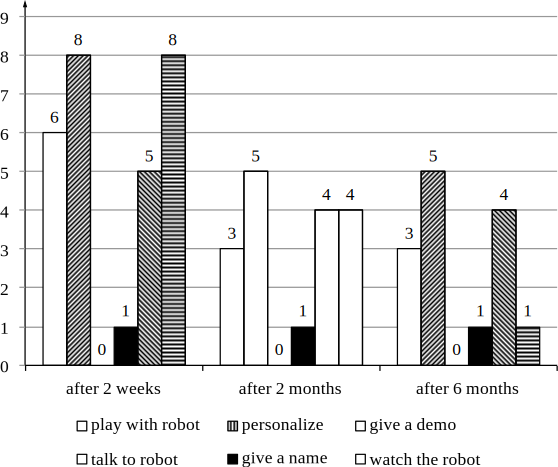
\includegraphics[width=10cm]{roomba-activities.pdf}% This is a *.jpg file
\end{center}
 \textbf{\refstepcounter{figure}\label{fig:roomba-activities} Figure \arabic{figure}.}{~~\small Over time there is a decrease of the social activities that households engaged in associated with the robot. Only 1 of the 9 households gave a name to their robot, and none of the households personalized their robot.}
\end{figure}

First, in terms of \textbf{anthropomorphic interactions} with the robot, we found that the effects were overall rather low and tended to fade out over time (first point is consistent with previous work by \cite{sung_housewives_2008}). Overall, we observed only few instances of people anthropomorphizing the robot or interacting with it in a human-social way. (Also, from the opposite point of view, the robot did not have a lasting social impact on the household, for instance, it did not lastingly change established cleaning roles.)
Some of the initially observed anthropomorphic interactions associated with the robot include \textit{watching} the robot for fun, giving a \textit{demo} of the robot to guests / visitors, \textit{personalizing} the robot, giving a \textit{name} to the robot, \textit{talking} to the robot using direct speech, and \textit{playing} with the robot. 
The majority of these anthropomorphic interactions with the robot did not last but participants stopped doing them after some time. Figure~\ref{fig:roomba-activities} shows how many of the 9 households engaged
in these activities during the 6 months when the study was conducted. We interpret that the nature of
human-robot interaction and how users experience the robot changes over time. We suspect that this is one of the reasons for why also the amount of
anthropomorphic / human-social interactions with the robot tends to decrease over
time. It is however possible that with some particular users, anthropomorphic interactions sustain.

\begin{figure}
\begin{center}
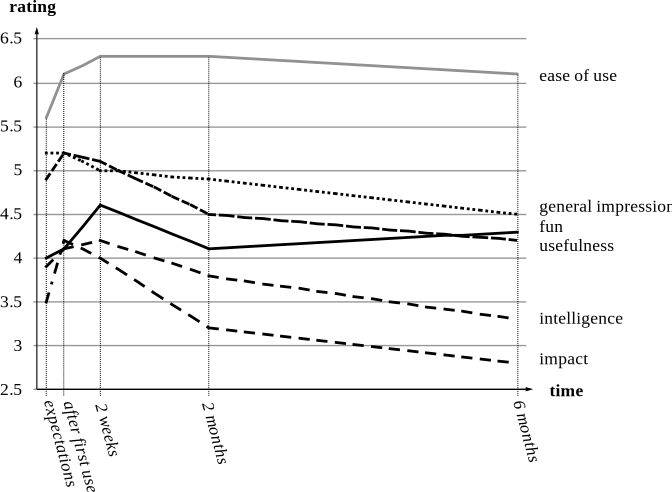
\includegraphics[width=14cm]{roomba-ratings.pdf}% This is a *.jpg file
\end{center}
 \textbf{\refstepcounter{figure}\label{fig:roomba-ratings} Figure \arabic{figure}.}{~~\small People's perception of the robot evolved over time, with stronger variations in the beginning. \textit{T1} = expectations, \textit{T2} = first usage, \textit{T3} = after 2 weeks, \textit{T4} = after 2 months, \textit{T5} = after 6 months.}
\end{figure}

Second, in terms of people's \textbf{perception of human-like characteristics and social traits of the robot}, we obtained similar findings. The robot was overall not perceived as having human-like characteristics, and attributions of intelligence, for instance, decreased over time.
At several time points during the 6-month lasting study, participants were asked to rate their perception and impression of the robot on 7-point Likert scales.
Concerning anthropomorphism, we included
\textit{perceived intelligence}, experienced \textit{fun} when using the
robot, and \textit{perceived impact} of the robot on the household as indicators for the perception of human-likeness in the robot. Figure~\ref{fig:roomba-ratings} shows how people's perception of the robot evolves over time.
Participants were generally not sure as how \textit{intelligent} they should rate the robot. Interestingly, at all five time points, male participants rated the robot as more intelligent (average 4.5) than females (average 3.4), however, this difference was not significant. Still, this suggests that gender, and probably other individual characteristics play a role. Also in terms of \textit{experienced fun} there was a non-significant but noteworthy gender difference. The rating for experienced fun remained quite stable for male participants, whereas it tended to decrease with time for female participants. The rating for \textit{perceived impact} reflects to what extent the robot is perceived to play a decisive role in the household. The average value remarkably increased after participants had used the robot the first time but then constantly decreased. This shows again, that people's perception of the robot changes over time, and that the initial moments using and interacting with a robot are special.
Overall, Figure~\ref{fig:roomba-ratings} shows that after the first usage of
the Roomba (T2), most of the perceived constructs slightly decrease (and hence
are less positively rated) as time goes by. The course is different for the
perceived \textit{ease of use} of the robot, as participants become more
experienced with the robot over time.

Summing it up, in accordance with previous work we also found relatively low rates of users
treating and perceiving their vacuum cleaning robot as a living (or human-like)
entity \citep{sung_housewives_2008}. We interpret that it might be the pure
functional purpose and non human-like form of the Roomba that prevented people
from anthropomorphizing it. Still, we observed some initial anthropomorphic
effects, both reflected in interaction with and perception of the robot.
However, most of the anthropomorphic effects did not last long. One fairly
stable human-like interaction with the robot was \textit{talking to the robot},
despite the fact that the robot was not able to recognize and respond to verbal
statements.

%%%%%%%%%%%%%%%%%%%%%%%%%%%%%%%%%%%%%%%%%%%%%%%%%%%%%%%%%%%%%
%
%
%
%		FORUM STUDY
%
%
%
%%%%%%%%%%%%%%%%%%%%%%%%%%%%%%%%%%%%%%%%%%%%%%%%%%%%%%%%%%%%%


\subsection{Forum Study: Anthropomorphism and the Purpose of Use of a Robot}
\label{sec:forum-study}


By carrying out a content analysis of 750 posts in three online discussion forums, we investigated the amount and context of anthropomorphic language that users apply when writing about their robotic dog AIBO, the vacuum cleaning robot
Roomba, and the tablet computer iPad \citep{fink_anthropomorphic_2012}. These three devices were chosen as they show different designs and
fulfill different purposes. We would describe (1) the AIBO as a zoomorphic /
pet-like robot that does not have a clear purpose but engages people to play
with it; (2) the Roomba as a mechanical / functional domestic service robot that has
a practical main purpose (vacuum cleaning) but offers not much of interactivity;
and (3) the iPad as a minimalistic designed interactive (touch-based) technology
with multiple purposes (both entertainment, and professional / practical use). The general goal of this analysis was to compare the three devices in terms of how much they are anthropomorphized in general and regarding the topic of the post. Furthermore, we wanted to find out where on a hypothetical scale of anthropomorphism the Roomba would range compared to the AIBO and the iPad.
There are two findings that are relevant here. 

First, in terms of how \textbf{anthropomorphic language is related to the device} (and most likely the overall design of it), we found a significant difference between how much the three devices are anthropomorphized. It was not a surprise that the highest amount of anthropomorphic
language (56.6~\%) was found in the AIBO forum. In comparison, only 11.7~\% and
respectively 2.2~\% of the segments in the Roomba and the iPad forum contained
anthropomorphic expressions. These data suggest that on a hypothetical scale of
perceived human-likeness (or rather life-likeness), Roomba is closer to the iPad
than to the AIBO, at least in matters of how they are described with words. This
was a surprised, as we had expected the Roomba would range closer to the AIBO, as both are autonomously moving robots. We interpret that the physical embodiment of the object and to what extent it resembles a life-like entity has a strong effect on how much it is anthropomorphized. This explains why a robotic dog is anthropomorphized more than more functionally designed devices.

Second, in terms of how \textbf{anthropomorphic language is related to the topic of the conversation}, we found a significant difference between the three topics \textit{relation}, \textit{usage}, and \textit{technical aspects}. The analysis suggests that anthropomorphizing happens more when the topic of conversation is \textit{relation}, compared to \textit{usage}, and \textit{technical} aspects. This was true for the Roomba and the iPad forum. However, in the AIBO forum, the amount of anthropomorphic segments was found highest for the \textit{usage} topic.  We interpret that it is the different type of interaction / context of use that makes the difference. Contrary to the iPad and the Roomba,
the AIBO is made to encourage the user in a playful / social interaction, which
in turn creates a specific use context. Further, AIBO has the ability to respond
intelligently to its user and environment, which might also encourage people to
ascribe human-like abilities to it while interacting with it.

Overall, findings of the forum content analysis suggest that there are differences in
people's tendency to use anthropomorphic language, originating form the design
characteristics of the artifact. A pet-like robot encourages people to use more 
anthropomorphic expressions when discussing about it in an online forum. However, 
the difference might also be related to other factors that we did not analyze 
here (\eg. author's characteristics). Our analysis further shows that the design 
of the robot seems to more important than the topic of the discussion. 
Interestingly, not only the physical embodiment
of the robot but also its interaction complexity and purpose of use are likely to play a role in how much the robot is anthropomorphized.

%%%%%%%%%%%%%%%%%%%%%%%%%%%%%%%%%%%%%%%%%%%%%%%%%%%%%%%%%%%%%
%
%
%
%		DOMINO STUDY
%
%
%
%%%%%%%%%%%%%%%%%%%%%%%%%%%%%%%%%%%%%%%%%%%%%%%%%%%%%%%%%%%%%


\subsection{Domino Study: Effects of Unexpected Robot Behavior}
\label{sec:domino-study}

The so-called ``Domino study'' describes a child-robot interaction study
that we carried out in a controlled lab setting. 13 pairs of 4-5 year old children (26 children in total) were playing a collaborative domino game, in which the robotic box ``Ranger'' \citep{fink_which_2014} was transporting domino tiles between the two children. 
The robot
was operated by one of the experimenters using the wizard-of-oz technique. For the first 7 times a child called the robot to come over to fetch a domino tile, Ranger behaved correctly, coming straight over to the child. However, in a second phase Ranger would show some unexpected misbehavior. This misbehavior was pre-defined and executed by the human Wizard at given time points. 
One of the goals of this
study was to investigate the effect of this unexpected robot behavior on (1) how much children ascribe
human-like abilities (\eg intentions, cognitive abilities) to the robot, thus how much they anthropomorphize it; and (2) children's interaction in general and their active engagement with robot. Children's perception 
of the robot was assessed in a qualitative way using several short-interviews, in which we assessed, for instance, to what extent children believed Ranger has its own will, has feelings, is able to understand what they say, can be left alone at home (the questionnaire was adapted by \citep{kahn_jr._robotic_2006}). The interaction data was analyzed quantitatively after having annotated the video recordings of the interaction. We were especially interested in typical human-like actions, \eg do children talk to it directly, use gestures 
toward it or use polite formulations.

First, regarding children's \textbf{perception} of the robot, we found that they commonly attributed hearing and seeing abilities to Ranger. However, though all children had interacted with a partly misbehaving robot, 12 of 26 children answered the robot would always obey to them, and the majority did not believe that the robot could do something silly. This suggests that they did not view the robot as having its own will or intentions itself. Most of the children attributed feelings to the robot and more than half of them could imagine Ranger as being their friend. This reflects that the robot is more perceived as a social agent but not necessarily having human-like qualities. In terms of what \citep{kahn_jr._robotic_2006} labels as ``moral standing'', we asked the 4-5 year-old's whether it would be ok to leave the robot alone at home while going on vacation. 20 of 26 children replied negatively, however their justifications on this answer do not reflect an attribution of moral standing to the robot (\eg that the robot deserves care).

\begin{figure}
\begin{center}

\includegraphics[width=7cm]{correlation.pdf}% This is a *.jpg file
\end{center}
 \textbf{\refstepcounter{figure}\label{fig:correlation} Figure \arabic{figure}.}{~~\small Correlation between children's anthropomorphic perception of the robot and their amount of interactions with it ($n = 13$ groups). A scatter plot of the count of engagement actions (per group) and the anthropomorphic perception of the robot (per group) shows a significant negative correlation ($r(11)=-0.56, p=.05$). There appears a cluster of groups at the top left corner, which suggests that those groups of children that interacted less with the robot, anthropomorphized the robot more in their verbal statements.}
\end{figure}

Second, the statistical analysis of the interaction data was unfortunately not very conclusive in terms of anthropomorphism. (This may be due to the fact that children showed very different \textbf{interaction styles}, so that we were not able to identify common patterns.) However, when looking at the amount of some specific actions toward the robot that reflect engagement, data suggest that children were more engaged with Ranger during the second phase (when the robot misbehaved from time to time). These engagement reflecting actions were \textit{exploring} the robot, using \textit{gestures} toward it, \textit{misusing} it, \textit{touching} the robot, \textit{talking} directly to it, and \textit{looking} at the experimenter (this shows that children were surprised and confused about the robot's misbehavior). We found that the manipulation of Ranger's behavior was sufficient to sustain children's engagement with the robot. This result is not directly related to anthropomorphism. However, we wanted to see whether there is correlation between children's engagement with the robot and how much they anthropomorphize it (perceive the robot as human-like, and attribute human-like characteristics to it). Do children who perceive more human-like characteristics in the robot also interact with it in a more human-like engaged way?
As Figure~\ref{fig:correlation} shows, the amount of children's anthropomorphic statements related to the robot (y-axis; qualitatively assessed from the interviews) and their interaction engagement with it (x-axis; quantitatively measured from the interaction videos) are negatively correlated $(r(11)=-0.56, p=.05)$. This was a main surprise. What had expected the opposite, namely children who engage more in the interaction would also perceive the robot as more human-like. However, the negative correlation suggests exactly the opposite: those children who interact more with the robot, treat and perceive it less as if it was a human. How can we interpret this finding? We think that those children who interacted more with Ranger, familiarized themselves better with it, and were better able to ``de-mystify'' the robot, thus being less in need of anthropomorphizing it.



Summing it up, children in the Domino Study anthropomorphized the robot conditionally: they attributed perceptual skills, mental states (feelings), and social companionship to the robot. Contrary, children did not attribute intention or moral standing to the robot. Some children tended to anthropomorphize the robot in how they were interacting with it: by using social or pointing gestures to it and by using polite formulations. Interestingly, we found a negative correlation between children's quantified engagement with the robot and their tendency to anthropomorphize the robot, which suggests that less interaction comes along with increased anthropomorphism.

%%%%%%%%%%%%%%%%%%%%%%%%%%%%%%%%%%%%%%%%%%%%%%%%%%%%%%%%%%%%%
%
%
%
%		ANTHROPOMORPHISM INDEX
%
%
%
%%%%%%%%%%%%%%%%%%%%%%%%%%%%%%%%%%%%%%%%%%%%%%%%%%%%%%%%%%%%%

\subsection{Anthropomorphism Index}
\label{sec:anthropomorphism-index}

It is not very clear how to operationalize and measure anthropomorphism. The phenomenon can be both subtle and complex at the same time, which poses challenges for finding appropriate study scenarios and metrics. 
So far, most studies on anthropomorphism involved showing pictures or videos of different types of robots to participants who are then asked to fill in a questionnaire (mostly using rating scales), in order to assess how much they perceived the different robots as human-like. We see two critical points here.
First, the \textit{evaluation scenario}, in which anthropomorphism is studied appears limited. When showing pictures or videos of robots to participants, the robots are not physically present and one cannot directly interact with it. This is critical, as the user experience may be blurred. We have seen in our own research that from seeing pictures or a video of a robot, participants were not able to make detailed judgments about the robot, concerning its height / size, the materials used in the robot, and the sounds it produces -- in other words, the whole expression of the robot was limited. The point we want to make here is that nothing is as rich as direct non-mediated interaction. Especially, if we agree that anthropomorphism arises in an interaction, we need to study it in evaluation scenarios that include interaction. Furthermore, it would preferable to study anthropomorphism over extended periods of time or over several interaction sessions, as we hypothesize that anthropomorphism shows dynamics over time (see Section~\ref{sec:dynamics}). 

Second, we also see limitations concerning the \textit{measurement aspect}. So far, there exist mostly questionnaires that quantify anthropomorphism using rating scales, such as the ``Godspeed'' questionnaire developed by \cite{bartneck_measurement_2008}. We are not sure, however, whether this is sufficient. Anthropomorphism is a social phenomenon and we question ourselves whether it can really be measured solely as a post variable and quantified on a closed rating scale that does not allow the participant to elaborate on his/her answer. There may be more qualitative alternatives by using open-ended more descriptive techniques, in order to better understand how exactly and why the participant perceives the robot as human-like. Also, questions may be less abstract but ask more specifically about concrete aspects of human-likeness, \eg as suggested by \cite{kahn_jr._robotic_2006,ruijten_introducing_2014}.

We propose that measurement tools of anthropomorphism should not only consider people's perception of the robot but also their interaction (how they behave) with the robot. Some previous work already suggests that there exists something like \textit{``anthropomorphic interaction''} \citep{krach_can_2008,hegel_understanding_2008,weiss_i_2009}. It would be interesting to formalize what this ``anthropomorphic interaction'' exactly is and how it can be evaluated and contribute to our understanding of anthropomorphism. Both quantitative and qualitative data could be combined for this, in order to reduce subjectivity.\footnote{In general, it is clear that the methods used need to be adapted to the specific research question. Large-scale surveys do usually not include in-depth interviews or physical interaction. However, for smaller sample sizes that one usually finds in empirical HRI studies, qualitative techniques allow for looking into details.}
We would like to take an initial step toward developing such a measurement tool by proposing the so-called \textit{Anthropomorphism Index} ($AntX$). This is on one hand a proposed toolkit to measure anthropomorphism related to a person, based on his/her perception of the robot and his/her interaction with it; on the other hand, it also stands for a value that reflects how much a person anthropomorphized a robot in a given interaction scenario. The idea, which is new here, is to combine aspects of the perception with aspects of the interaction (in-situ measurement). This builds on the idea that anthropomorphism is a social phenomenon that arises in an interaction.

Typically, \textbf{perception} would be measured both prior to the interaction (expectations of human-likeness of robots in general, for instance) and after the interaction with the robot (describing and viewing the robot as human-like). A list of concrete questions is not defined yet but examples could be taken from already existing questionnaires (\eg \cite{bartneck_measurement_2008,weiss_i_2009,kahn_jr._robotic_2006,ruijten_introducing_2014}).
There can be yes/no type questions (\eg ``Can the robot be hungry?''; ``Can the robot feel ashamed?''), ratings using semantic differentials or Likert-type scales (\eg ``Playing with the robot is more like ... `playing with a toy' compared to `playing with a friend'.'' (semantic); ``The robot understands me'' (1-5 Likert-scale, for instance)), and open-ended questions (\eg ``Can you leave the robot alone at home while going on a 2-week holiday? Why (not)?''). The respective answers to these questions can be assigned with points reflecting the degree of anthropomorphic perception, and then summed up to obtain an overall estimate.

The \textbf{interaction} scenario should be video-recorded to allow for later analysis. Specific types of anthropomorphic interaction (\eg use of polite formulations and direct speech, establishing eye-contact with the robot) can then be annotated in the videos. A list of such specific actions is not yet defined. Again, there can be yes/no items (\eg Did the participant use polite formulations or other forms of social desirability toward the robot?), and more quantified items (\eg How much did the participant talk directly to the robot?, How much did the participant establish eye-contact with the robot?). It would also be interesting to look more into details of the behavior aspects, for instance, How did the participant address the robot verbally?, How much was the participant using normal human-human like conversation as compared to typical interface-like conversation (more giving commands, adjusting speech rate, using monotonic speech). One could again think of assigning a specific number of points for items that reflect anthropomorphic interactions, and in the end build the sum to obtain an overall estimate.

For both values, perception and interaction, there may be a pre-defined maximum value of $AntX$ or a fixed range of it that is seen as the desired degree of anthropomorphism (maximum anthropomorphism may not always be optimal or desired, sometimes a more machine-like treatment is preferred). In case of several interaction sessions or longitudinal interaction, several short interviews / questionnaires could be carried out to track how perception changes over time. Accordingly, the video analysis can be segmented and split into phases, which are then compared against, so to analyze how anthropomorphic interactions evolve over time.



%\section{Related Work}
%\label{sec:related-work}
%
%Findings from related work, maybe theoretical background.

%%%%%%%%%%%%%%%%%%%%%%%%%%%%%%%%%%%%%%%%%%%%%%%%%%%%%%%%%%%%%
%
%
%
%		OUR IDEAS
%
%
%
%%%%%%%%%%%%%%%%%%%%%%%%%%%%%%%%%%%%%%%%%%%%%%%%%%%%%%%%%%%%%


\section{Extensions to the Understanding of Anthropomorphism in HRI}
\label{sec:our-ideas}

As presented in the previous section, some of our research on anthropomorphism in HRI produced unexpected results. We see it as our job to not hide surprising results but to offer a plausible interpretation to the scientific community.
To allow doing so, we went through literature on anthropomorphism and reviewed articles from various disciplines, including HCI, philosophy, developmental and social psychology, cognitive sciences, artificial intelligence, and neurosciences.
It is not trivial to synthesize and summarize such a diverse body of literature. Overall, we found that, on one hand anthropomorphism is an interesting research topic in a variety of disciplines. On the other hand, researchers agreed that anthropomorphism is of complex nature and that the phenomenon is still not very well understood as a whole \citep{duffy_anthropomorphism_2003,epley_seeing_2007}.
The literature review helped us not only to better interpret our unexpected results on human-like engagement with robots but also to get an idea of the psychological motivations and underlying cognitive processes of anthropomorphism \citep{epley_seeing_2007}. We think that it is worth sharing the obtained insights with the broader HRI community (which is diverse itself).
To do so in a structured way, we would like to make three suggestions toward extending the current understanding of anthropomorphism in HRI. We do not offer a perfect model or a complete framework here but share our conceptual ideas. This will hopefully lead to a constructive discussion among researchers and help generate more empirical work on why humans tend to perceive and interact with robots as if they were somewhat human. 

%%%%%%%%%%%%%%%%%%%%%%%%%%%%%%%%%%%%%%%%%%%%%%%%%%%%%%%%%%%%%
%
%
%
%		MULTIPLE FACTORS
%
%
%
%%%%%%%%%%%%%%%%%%%%%%%%%%%%%%%%%%%%%%%%%%%%%%%%%%%%%%%%%%%%%


\subsection{Anthropomorphism is based on Multiple Factors}
\label{sec:multiple-factors}

%\begin{figure}
%\begin{center}
%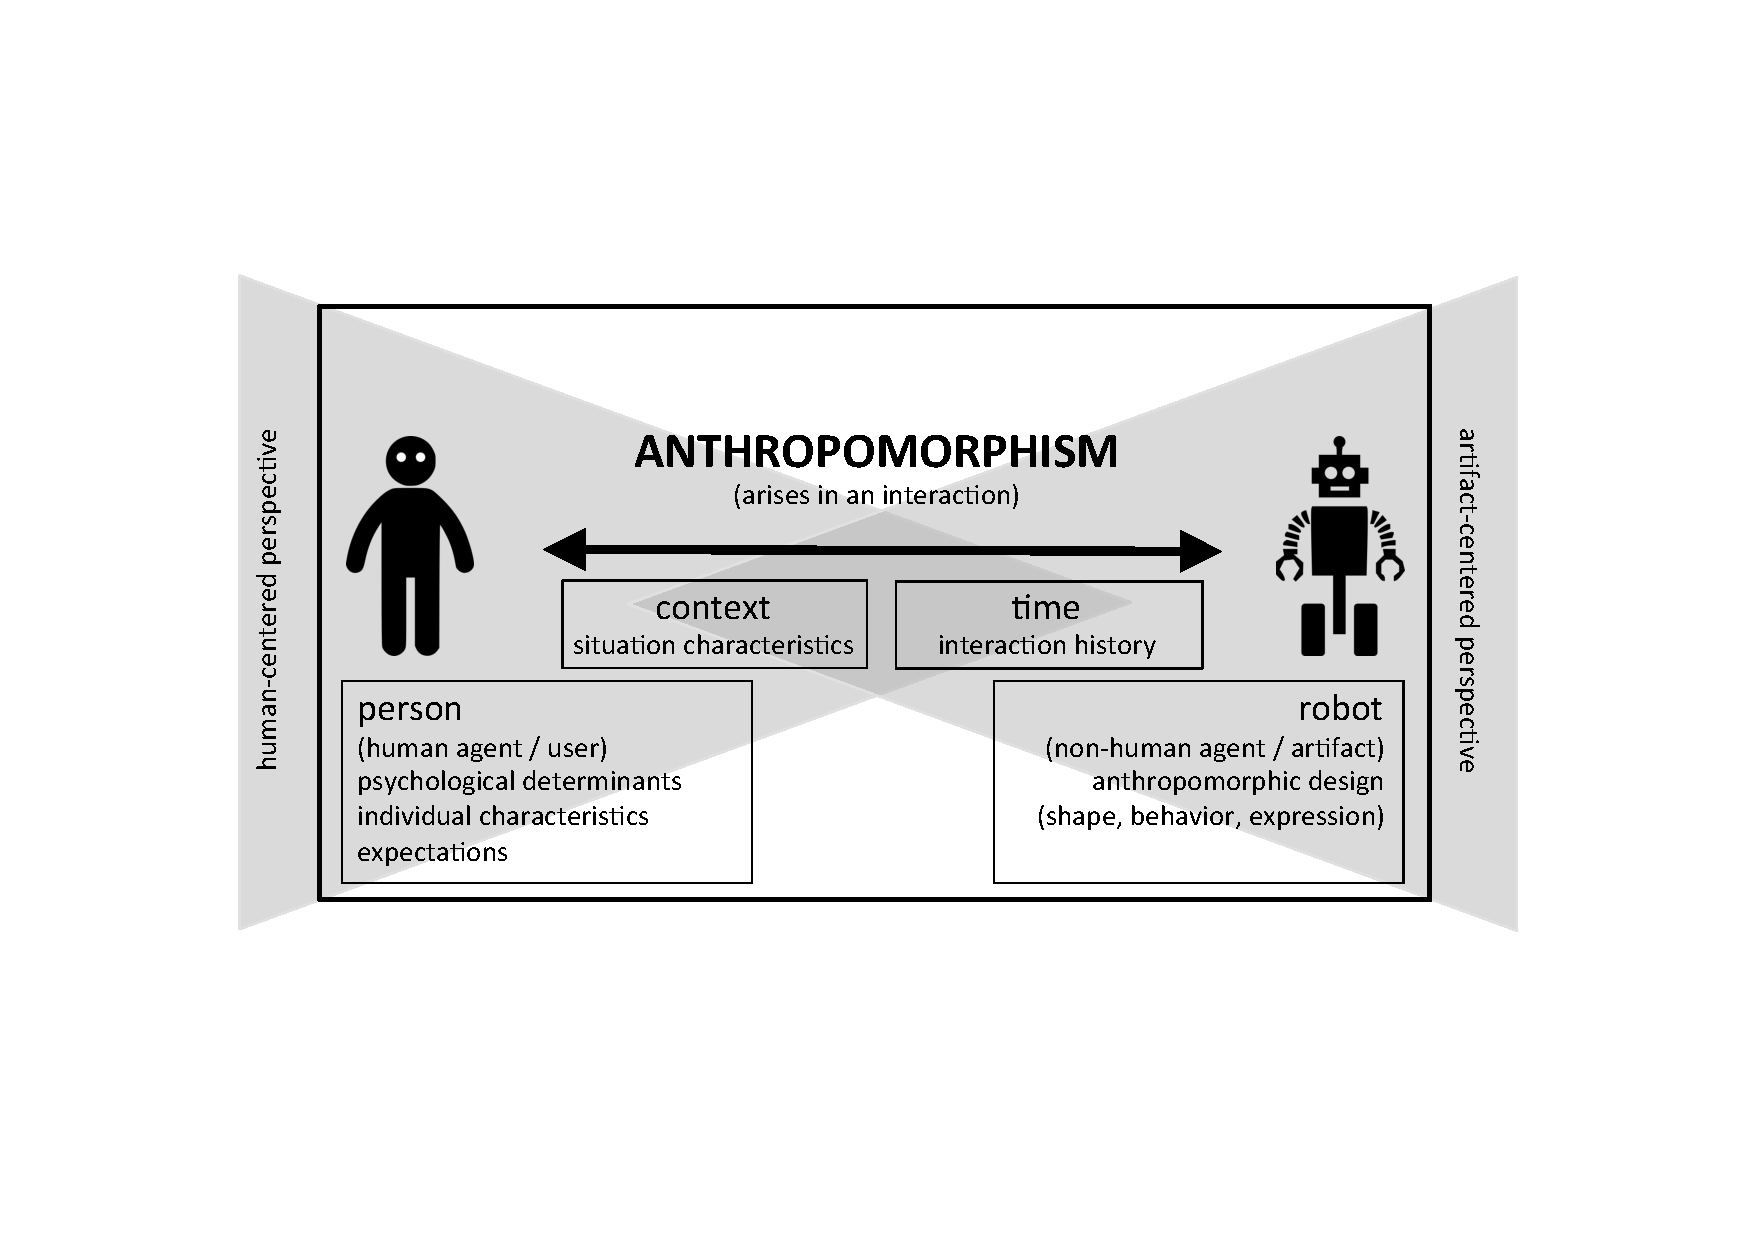
\includegraphics[width=13cm]{anthropo.pdf}% This is a *.jpg file
%\end{center}
% \textbf{\refstepcounter{figure}\label{fig:multiple-factors} Figure \arabic{figure}.}{~~\small Anthropomorphism arises in an interaction between a human ($H$) and a robot ($R$) in a specific context of use ($C$). These are the three main factors on which anthropomorphism is based. Further, to account for dynamics over time ($t$), the interaction history is taken into account. There are two main perspectives from which anthropomorphism can be studied, a human-centered one, focusing on variables related to the human; and an artifact-centered one, focusing on variables related to robot.}
%\end{figure}

Once considering anthropomorphism as a phenomenon that arises in an \textbf{interaction} between a robot and a human in a given context \citep{persson_anthropomorphism_2000}, it becomes apparent that the phenomenon is based on multiple factors.
%(see Figure~\ref{fig:multiple-factors}).
To account for both the human and the robot as the two main interaction partners, as well as for the context and other external variables that constitute the interaction, a comprehensive perspective is required. We suggest to apply the concept of \textbf{user experience} to interpret how anthropomorphism emerges. According to ISO 9241-210, user experience is defined as \textit{``a person's perceptions and responses resulting form the use and/or anticipated use of a product, system or service''}. User experience includes all the users' emotions, beliefs, preferences, perceptions, physical and psychological responses, behaviors and accomplishments that occur before, during and after use. The ISO also names three factors that influence user experience: system, user, and the context of use \citep{iso_ergonomics_2010}.
Applying such a user-centered perspective, we take up the \textbf{human} (denoted as $H$), the \textbf{robot} ($R$), and the \textbf{context of use} ($C$), as the three main factors on which anthropomorphism (denoted as $A$) is based.

\subsubsection{Characteristics of the Human\\}
\label{sec:factor-human}

The first main factor of anthropomorphism are characteristics of the human $H$. This includes several sub-factors $(h_0, ... , h_n)$, \eg psychological factors, demographic factors, and other traits of personality. 
It would theoretically be possible to compute a human-specific value $H=\{h_0, ... , h_n\}$ that indicates how much a person is likely to anthropomorphize, based on individual factors (in practice this looks different). Such value could for instance range between $0$ and $1$ to suggest something similar to a probability for a person to anthropomorphize.
The point here is to account for individual differences of anthropomorphism and to acknowledge that each user is unique, having individual expectations, beliefs, emotions, and conceptions. This can be called a \textit{human-centered perspective} on anthropomorphism. 
%(see Figure~\ref{fig:multiple-factors})
In the following paragraphs we present possible sub-factors. This list may not be complete, and we leave it open to other researchers to extend it.
 
\paragraph{Psychological factors} can account for why some people are (intrinsically) more motivated to anthropomorphize than others. Irrespective of a robot's characteristics (which will be treated in the next Subsection, \ref{sec:factor-robot}) three main psychological determinants have been identified to explain a person's readiness to anthropomorphize. \cite{epley_seeing_2007} present those in their \textit{3-Factor Theory}, which suggests that some people are more likely to anthropomorphize when:

\begin{enumerate}
\item anthropocentric knowledge is accessible and applicable to the artifact (\textit{elicited agent knowledge})
\item they are motivated to explain and understand the behavior of other agents (\textit{effectance motivation}), and
\item they have the desire for social contact and affiliation (\textit{social motivation}).
\end{enumerate}

The first factor, \textit{elicited agent knowledge}, is a \textit{cognitive determinant} of anthropomorphism and based on the idea that a person builds a mental model of the other agent (we treat this aspect in more detail in Section~\ref{sec:cognitive-viewpoint}). In short, the central point here is, that the person uses knowledge (a mental representation) about other humans (or him/herself) to make inferences on the (unfamiliar) robot. Anthropocentric knowledge is an easy source for us because as a human being we experience the world ourselves, as a human, and not as something or someone else. We have no other experience than the self, so in turn we tend to draw conclusions from ourselves on others' mental states. Attributing our own states to other humans is called ego-centrism. This mechanism is particularly formed in young children and decreases with cognitive development and the learning to distinguish the self from other humans, and non-human agents.

The second factor, \textit{effectance}, as well as the third factor, \textit{sociality}, are \textit{motivational determinants} of anthropomorphism. \textit{Effectance} is understood as one's motivation to interact effectively within one's environment and the agents that inhabit it. In other words, we are motivated to make sense of our environment, and to be able to understand, predict and reduce uncertainty. According to \cite{epley_seeing_2007}, \textit{effectance motivation} can lead to anthropomorphize because this serves to reduce uncertainty and increase comprehension (especially about unfamiliar stimuli). It becomes apparent that people who feel more uncertain within their environment are likely to be more prone to anthropomorphize.

The third factor, \textit{sociality} describes a person's motivation for social contact, social connection, and social approval from other agents. In lack of social connections to other humans (\eg friends, family, colleagues), a person is more likely to compensate these social connections by anthropomorphizing non-human agents. Interestingly, the two most commonly anthropomorphized non-human agents that serve to compensate for social connection to humans are pets and religious agents \citep{epley_seeing_2007}. In short, the motivation to be socially connected increases the tendency to anthropomorphize for two reasons. On one hand, sociality motivation increases the likelihood to perceive human-like characteristics in non-human agents; on the other hand, it also increases the tendency to search for sources of social connection in one's environment.


\paragraph{Demographic factors} typically involve (but are not limited to) age, income aspects (often referred to as `social class'), cultural affiliation, and gender. Related work suggests that some of the demographic factors may impact to what extent a person is likely to anthropomoprhize. For instance, children tend to anthropomorphize especially robots more than adults.\footnote{It is not clear whether children really anthropomorphize more or whether they are just more prone to using metaphors within their conception of the world, or to projecting their own emotional states on any artifact that behaves with a certain independence.} Also, some cultures are notorious for their anthropomorphic religions and worldviews \citep{epley_when_2008}, and previous work suggests that anthropomorphism is a culture-sensitive phenomenon \citep{kaplan_who_2004,bartneck_cultural_2005}. 


\paragraph{Other person-related aspects} also play a role in shaping user experience, as well as probably for anthropomorphism. For instance, it has been found that expectations and attitudes toward using a robot can impact on how the robot is experienced and interacted with \citep{forlizzi_service_2006,forlizzi_how_2007}. In one of our studies, we also found that, those children who expected a robot to be very human-like, tended to be more disappointed as they discovered the limitations of the actual non human-like robot that we were using for the interaction study.\footnote{Due to a rather small sample size, we were unfortunately not able to identify the impact of the initial expectation on anthropomorphism.} Similarly, also previous experience with robots in general, knowledge about robots, and professional background is likely to play a role. Users who are better able to estimate the capabilities of the robot may be less likely to anthropomorphize the robot.


\subsubsection{Characteristics of the Robot\\}
\label{sec:factor-robot}

The second main factor of anthropomorphism are characteristics of the robot $R$. Similar to before, this includes several sub-factors $(r_0, ... , r_n)$, \eg the robot's form, including its physical shape (how it looks like), materials, and other features of the design\footnote{Note that `design' may not only refer to the physical shape of a robot but to the total expression that it has as an artifact \citep{bartneck_shaping_2004}. Similarly, \cite{disalvo_hug:_2003} uses the term `form' to refer to both the physical shape, materials, and behavioral qualities of a product. In this article, we use `form' interchangeably to `physical shape' and `design' to embrace also behavioral and functional aspects. Thus, `form' is one aspect of the `design'.}, such as its interactions through expression, communication and behavioral qualities, and its functionality. If we are able to measure and evaluate these sub-factors regarding their similarity to human-likeness (or even applying a dyadic yes-or-no decision), we could obtain a robot-specific value $R=\{r_0, ... , r_n\}$ that indicates how much the robot is likely to be anthropomorphized by a user. Also this value may range between $0$ and $1$, with $1$ being a human. The point here is to account for differences between the given characteristics of different robots. As such, this main factor applies an \textit{artifact-centered} perspective on anthropomorphism
%(see Figure~\ref{fig:multiple-factors})
, as it argues that there are features of the artifact that suggest to the human to perceive it and treat it as if it had some human-like qualities.

\paragraph{The Physical shape} of a robot refers to `how the robot looks like' and includes its general form, and other visible features, such as its size, the materials used, its color, and specific details. Generally, robots can be divided into human-like (anthropomorphic) and mechanical (non-anthropomorphic) robots. However, it makes sense to be slightly more specific about the form, and \cite{fong_survey_2003} suggest four categories: anthropomorphic, zoomorphic, caricatured, functional. The borders and transitions between these categories are not very well defined. 
Of particular importance seems to be the presence or absence of specific human body parts, such as arms and hands, legs, a torso or a head and face. Of those, the faces of robots have received remarkable attention concerning how they are perceived and accepted. \cite{disalvo_all_2002} studied what features and dimensions of a humanoid robot's face most dramatically contribute to people's perception of its humanness. The authors analyzed 48 humanoid robot heads and found that the presence of certain features, the dimensions of the head, and the total number of facial features heavily influence the perception of humanness in robot heads. 

Interestingly the authors found that despite the fact that all of the 48 evaluated robot were classified as humanoid, the majority of them was not rates as being very human-like by the participants. This result does not conflict with the robots being classified as humanoids, for that simply means that their form resembles a human more than it resembles any other form. It does, however, \textit{``raise the issue of how human-like a robot can be perceived by form alone''}. \citep{disalvo_all_2002} interpret that the `humanness' of a robot is defined not only by form but interactions through expression, communication, and behavior. We treat these aspects as a separate sub-factor of the robot's characteristics.


\paragraph{Expression, communication, and behavior} refers to how the robot expresses its human qualities through interacting and behaving. In fact, many humanoid robots express their human-likeness not in physical shape but only through the \textit{suggestion} of features \citep{disalvo_all_2002}. Besides this, communication and interaction modalities of a robot are likely to play a role to what extent the robot will be anthropomorphized. Can the user interact with the robot through a touch interface, or using speech? Does the robot respond using linguistic utterances or non-linguistic sounds? Is the voice human-like or synthetic, on-board or coming from an external second device? A study by \cite{takayama_im_2009} found that this has an effect on people's perception of trust in the robot and how convincing the robot appears to them. Besides this, we expect that a robot's behavioral aspects concerning human-social interaction have an impact. Does the robot use polite formulations, etiquette, appropriate facial expressions? Are its responses and reactions timely? Usually, robots that directly interact with humans are slow, which appears not very human-like to most participants. 

\paragraph{The functionality, and purpose} are a robot-related characteristic that also partly determines the context of use. This aspect includes what kind of expectations the user may have of the robot, and how the user imagines using the robot. Is there only one user or a group of people interacting with the robot at the same time? Is the purpose of the robot a playful or a serious one? Does the robot have a purpose at all \citep{kaplan_free_2000}? We come back to this aspect in the next section, related to the context of use.



\subsubsection{Characteristics of the Context of Use\\}
\label{sec:factor-context}

\textit{Context of use} is defined by the ISO as \textit{``users, tasks, equipment (hardware, software and materials), and the physical and social environments in which a product is used''}. Accordingly, there are various aspects that can impact how a robot is experienced. The real or imagined \textit{purpose} of a robot, including the application context in which it is typically used (\eg office environment, home, rehabilitation center, public space, \etc) as well as the task context (\eg serious or playful task; composition of human-robot team; number of users) and the (social) role in which the robot is used / experienced are taken into account. Generally, when the context of use of a robot is social, entertaining or playful, it will enhance anthropomorphism, compared to when the context is a routine or focused serious task (security, rescue, \etc). \cite{joosse_what_2013} showed, for instance, that when the same robot (NAO) was used in a different task context (cleaning task \vs tour guide), users ascribed different personalities to the robot. Also our content analysis of online discussion forums (see Section~\ref{sec:forum-study}) shows that the purpose of the robot has an impact on the amount of anthropomorphic descriptions. Also Goetz and Kiesler's work revealed a link between a robot's context of use and people's perception of the robot. The authors found that people prefer a serious robot for serious tasks and a less serious robot for more playful tasks \citep{goetz_cooperation_2002,goetz_matching_2003}. \cite{kaplan_free_2000} discussed the role of uselessness in the design of robots. The author argues that artificial pets like AIBO have no real purpose, in a sense that they do not provide any kind of service or, in other words, \textit{``they are not doing what you tell them to do''} and \textit{``they might refuse the order of its owner''}. It may be this very aspect that increases people's tendency to anthropomorphize the robot. According to Kaplan, it is in our daily use language that we tend to attribute intentions to devices that are not doing their job well. For instance, we do usually not develop a relationship with our computer, washing machine or TV set when they work just properly; however, when they start dis-functioning, when they show that they can act differently than what we ordered, then we are ready to ascribe to them so kind of \textit{intentionality}. This aspect lies somewhat in between the characteristics of the robot (its behavior) $R$ and the context of use $C$.

The characteristics of the context can also impact on the user experience and in turn foster or hinder anthropomorphism indirectly. For instance, when there are several friends of the main user interacting simultaneously with the robot, the likelihood of anthropomorphism may be increased. The context here is already social when several people who know each other engage in social interaction among themselves, so the robot may be perceived as being somewhat part of the social interaction, and hence it may be attributed human-social qualities \citep{baxter2013do}.


%%%%%%%%%%%%%%%%%%%%%%%%%%%%%%%%%%%%%%%%%%%%%%%%%%%%%%%%%%%%%
%
%
%
%		MULTIPLE LAYERS / LEVELS
%
%
%
%%%%%%%%%%%%%%%%%%%%%%%%%%%%%%%%%%%%%%%%%%%%%%%%%%%%%%%%%%%%%

\subsection{Anthropomorphism has Multiple Layers (Levels)}
\label{sec:multiple-layers} 

Despite a fairly huge body of literature on anthropomorphism, the phenomenon is still not very well understood. \cite{persson_anthropomorphism_2000} argued that one of the issues is the scientific community's lack of sufficient understanding of the wide range of phenomena that anthropomorphism encompasses. More specifically, the authors argued that anthropomorphism \textit{``is not one phenomenon''} but \textit{``means different things on different levels''}. This viewpoint appears to make sense, as also human-likeness itself is not `one big concept' but consists of a huge variety of details, it is multifaceted and complex itself, so there may also be not just one single type of anthropomorphism but different levels, layers or gradations. Accordingly, \cite{persson_anthropomorphism_2000} propose to understand anthropomorphism as a multi-layered phenomenon, that arises in different levels. The authors list six levels, that each have their own characteristics and involve specific types of user expectations. The suggested levels are \textit{primitive categorization}, \textit{primitive psychology}, \textit{folk psychology}, \textit{traits}, \textit{social roles} and \textit{emotional anthropomorphism}. They suggest to use this multi-layered schema as a tool for analyzing systems with respect to anthropomorphic effects.
Similarly, also \cite{ruijten_introducing_2014} propose to not see anthropomorphism as one big phenomenon that is either \textit{their} or \textit{not their}. In contrast to \cite{persson_anthropomorphism_2000}, they suggest to understand anthropomorphism as a continuum, ranging from ow to high levels, depending on how much the attributed characteristic is typically or uniquely human (see Figure~\ref{fig:mental-model-overlap}).


\begin{figure}
\begin{center}
\includegraphics[height=5cm]{mm-overlap.pdf}% This is a *.jpg file
\end{center}
 \textbf{\refstepcounter{figure}\label{fig:mental-model-overlap} Figure \arabic{figure}.}{~~\small When we anthropomorphize a robot, our mental model of the robot overlaps to some extent with our mental model of a human. This is to provide an explanation to ourselves for how the unfamiliar aspects of the robot work the way they do. The overlapping part may vary, depending on how similar the two mental models of the robot and the human are. Also, other mental models, \eg the one of a dog or a computer, may play a role (this is not displayed here). Note further that we may not have one general mental model of a human but that we may have several and more specific models of certain actions (how a human reaches and grasps a cup) and behaviors (how a dog conveys that he wants to play), for instance.}
\end{figure}

\nocite{admoni_multi-category_2012}

\subsubsection{A cognitive viewpoint on anthropomorphism\\}
\label{sec:cognitive-viewpoint}

Anthropomorphism has a fundamental `sense-making' function \citep{persson_anthropomorphism_2000}. It involves a cognitive process of induction whereby \textit{``people reason about an unknown stimulus based on a better-known representation of a related stimulus''} \citep{epley_when_2008}. This is important. The particular process of reasoning on which anthropomorphism is based includes two central aspects.
First, it requires \textit{``an unknown stimulus''} and a \textit{``better known representation of a related stimulus''}.\footnote{We suspect that anthropomorphism can also occur in absence of such unknown stimuli. Then, rather individual psychological factors may play a role (instead of applying a cognitive explanation). For instance, individuals who lack social connection to other people \citep{epley_creating_2008} tend to anthropomorphize objects despite the fact that they may have an accurate mental model of the object. This may then be a more ``projection''-type of anthropomorphism, which does not necessarily serve to explain something unknown.} Humans generally tend to use the closest (most similar) better known mental representation in order to explain the unknown stimulus. (This better known available representation must not necessarily be the one of a human, however, it is often the case because what we understand best in this world is ourselves.)
A second central aspect is a person's \textit{Theory of Mind} -- the ability to attribute mental states (\eg beliefs, intentions, knowledge, desire) to oneself and others, and to understand that others' states are different from one's own.

\nocite{hegel_theory_2008}

\begin{figure}[!b]
\begin{center}
\includegraphics[height=3.5cm]{low-high.pdf}
\end{center}
 \textbf{\refstepcounter{figure}\label{fig:low-high} Figure \arabic{figure}.}{~~\small Anthropomorphism is not discrete being either \textit{there} or \textit{not there} but may be a continuum, having lower and higher levels, based on how much the attributed characteristic is typically or uniquely human (illustration adapted by \cite{ruijten_introducing_2014}).}
\end{figure}

There are two possibilities how anthropomorphism can be multi-layered from a cognitive point of view.
First, in the case of anthropomorphism, a person chooses their mental model (or parts of it) of a human (the `better known representation') in order to explain some aspect about the robot (the `unknown stimulus'). In other words, the mental model that the person has of the robot is to some extent similar to the mental model that he/she has of a human (see Figure~\ref{fig:mental-model-overlap}).
We suppose that regarding anthropomorphism, it matters to what extent the mental model of the robot is based on the mental model of a human (for instance, is it fully identical, only partly, not at all?).
Thus, how much thus the overall mental model of the robot overlap with the mental model of a human? How many specific actions / traits of the robot are explained by resorting to a human-like representation of it?

Second, the characteristic of being multi-layered is also based on how typically or uniquely human the attributed characteristic is (see Figure~\ref{fig:low-high}), how much `cognitive depth' it implicates. For instance, attributing animacy, perceptual skills, or primary emotions (\eg fear, anger, sadness, happiness) to a robot are an example for a lower level anthropomorphism. These attributions are not uniquely human and reflect a less deep cognitive process. In contrast, the attribution of intent, moral standing, or secondary emotions, such as desire, shame or guilt are an example for higher level anthropomorphism. These attributions come from more complex chains of thinking. We suggest three cognitive stages that are not mutually exclusive but overlap (also in terms of temporal dynamics of anthropomorphism, Section~\ref{sec:dynamics}).

Based on this cognitive viewpoint, 
we propose that anthropomorphism is multi-layered \citep{persson_anthropomorphism_2000}. This means that anthropomorphism is not either `there' or `not there' but that there exist multiple layers of it, to which we will refer to as \textit{lower and higher levels of anthropomorphism}. The different levels (it may also be a continuum) are based on different cognitive correlates. 
\textbf{Lower level anthropomorphism} is based on a less thorough mental processing of an interaction. It can be more spontaneous and unmindful. This type of superficial reasoning about the robot may be predicated on specific cognitive correlates.
Contrary, \textbf{higher level anthropomorphism} typically involves a profound thoughtful mental processing of the interaction as well as deeper reasoning about the robot. We assume that also such deeper interactions are based on specific cognitive correlates (see Section~\ref{sec:cognitive-correlates}).


\subsubsection{Cognitive Correlates of Anthropomorphism\\}
\label{sec:cognitive-correlates}

The following paragraphs provide an initial interpretation of anthropomorphism in terms of \textit{cognitive correlates}: How can human cognition explain the dynamic nature of our interactions with robots? What are the main cognitive stages upon which researchers can build to design `deeper' human-robot interactions?
A cognitive viewpoint on anthropomorphism is important because people's
estimation of an agent's knowledge model and its capabilities affects the way
they relate to it. This holds implications for the resulting interaction with
the system, the user experience, and the acceptance. Previous research examined
the validity of the mental model concept with various kinds of robots
\citep{schmitz_concepts_2011,kiesler_mental_2002}. Findings suggest that people
tend to hold richer mental models of anthropomorphic robots in contrast to
mechanic ones \citep{kiesler_mental_2002}.
%\footnote{Later in this article,
%we may however come to question how far this result is based on
%expectations from the human user side, which are likely to be refined
%after continued interaction, and after the user gets acquainted with the
%robot's behavior.}
A similar finding is described in
\cite{hegel_understanding_2008} and \cite{krach_can_2008}. In a user study using
functional magnetic resonance imagery (fMRI), the authors found that
participants implicitly attributed human-like qualities, such as mental states,
to their non-human interaction partner. Indeed, from an early age humans develop
a tendency to explain one's own and others' actions in terms of beliefs, desires
and goals, called \textit{Theory of Mind}. Theory of Mind allows the
implicit attribution of intentions and other mental states to others
\citep{premack1978does,leslie_pretense_1987,Frith2003}. The finding of
\cite{hegel_understanding_2008} and \cite{krach_can_2008} was evident at the
behavioral level as well as on the neuro-physiological level: the more the
human-likeness of the artifactual partner increases, the more brain areas
associated with Theory of Mind get activated \citep{krach_can_2008}.
Implication of human brain area involved in the inference of others' mental
states has also been shown in response to viewing
non-anthropomorphic / non-humanoid robotic gadgets whose behavior has been
described as unpredictable -- but not in response to those whose behavior was
described as predictable -- a finding also found at the behavioral level
\citep{Waytz2010}. Interestingly, the grey matter volume of a brain area
related to Theory of Mind has been correlated to individual's score of
anthropomorphism \citep{cullen2013individual}.

At a lower, more automatic, level, robots have been shown to elicit resonance
behaviors in the human brain. Resonance behaviors \citep{Rizzolatti1999} are
mechanisms by which the brain areas involved in the internal representations of
an action, an emotion or a sensation are equally recruited during the perception
of another individual performing the same action or experiencing the same
emotion or sensation. The neurons showing resonant properties have been called
mirror neurons and have been found in a wide range of modalities (motor,
emotional \etc). Seeing a robotic arm reaching for an object
activates the motor mirror neurons the same way as for seeing a human arm
reaching for the same object \citep{Gazzola2007,oberman_eeg_2007}. However, a
study of emotion perception on a robotic face, found reduced activity in
emotional brain area known to have mirror properties in response to the robotic
face compared to a human face \citep{Chaminade2010}. Nevertheless, the authors
showed that when participants were explicitly instructed to pay attention to
the robot's emotional expression, motor mirror neurons got activated.
Interestingly, using electroencephalography, it has also been shown that
emotional behavior elicited by a robot face influences the speed of human
responses as well as early brain processes the same way as emotional expression
of a human face did \citep{Dubal2010}.


%


In sum, this branch of research suggests that anthropomorphism implies that
people thoughtfully develop a mental model of agents in their environment and
that they make inferences about these agents based on what is familiar to them
-- themselves, humans and human behavior.
%This understanding builds on the
%theory of mind,  a
%person's ability to attribute mental states to oneself and others. 
%A theory of mind for other agents enables us to attribute intentionality to those agents \citep{leslie_pretense_1987,admoni_multi-category_2012}. 
We briefly reviewed neuro-physiological evidence of a link between the tendency
to thoughtfully anthropomorphize and the engagement of brain processes involved
in the attribution of mental states to other humans. The human-likeness quality
of the artifactual agent seems to play a role in the involvement of Theory of
Mind but also the unpredictable feature of the agent behavior alone seems to be
sufficient. Low-level mechanisms of the brain that allow humans to map others'
motor behaviors into their own repertoire are equally elicited when perceiving a
robot's action. It is not yet clear whether humans are processing emotional
signals from a robot the same way as they do for human beings. 


\subsubsection{Cognitive Processes and Stages\\}

Based on these lower and higher level cognitive correlates that lead to different levels of anthropomorphism, we would like to propose three main cognitive processes / stages that are relevant for interpreting the level (`depth') of anthropomorphism that is observed.

%\hl{Infrahumanization theory}: people differentiate the ingroup from other groups by attributing uniquely human emotions. They consider secondary (uniquely human) emotions as being more characteristic of their own group than of the outgroup (Leyens, et al., 2000).\\
%Typical \textbf{primary emotions} include fear, anger, sadness, and happiness (although these can also be felt as secondary emotions). \textbf{Secondary emotions} appear after primary emotions and may come from more complex chains of thinking. Examples: longing, affection, envy, shame, guilt).

\textit{Stage 1} is the instinctive, pre-cognitive identification of living peers. Studies conducted by \cite{rosenthal-vonderputten_experimental_2013}, who investigated the neural correlates of emotional reactions of humans towards a robot, support the idea that humans tend to anthropomorphize robots intuitively in this pre-cognitive way. \textit{Empathy} is characteristic of this stage \citep{rosenthalvonderPutten2013neural}. At \textit{Stage 1}, intuitive anthropomorphism is likely at a lower level: so-called mirror neurons get automatically activated in response to the participant viewing the robots' actions and reacting emotionally toward it. This process may be similar to two previously described perspectives.
First, relating this cognitive \textit{Stage 1} to a specific \textbf{user experience}, it may be similar to what \cite{norman_emotional_2003} characterizes as the \textit{visceral level}. By this, he means the first impression that a person has of a product, based on experience. At this level, people do not think about the product but make spontaneous judgments.
Overall, Norman lists three different levels, that stand for different user experience dimensions, when analyzing     how people experience using a product for the first time and getting emotionally attached to it. Emotional attachment to a product is somewhat related to anthropomorphism. We come back to the other two levels of user experience later on.
Secondly, our proposed cognitive \textit{Stage 1} may also be similar to what \cite{takayama_perspectives_2012} calls the \textit{in-the-moment} perspective on agency with a robot (in contrast to the \textit{reflective} perspective). For instance, when reflecting upon it, we may \textit{not} perceive agency in a social robot, however, this may feel quite differently right in the moment of interacting with the robot.
Takayama argues that neglecting to separate reflective perspectives from in-the-moment perspectives of agency is one of the major sources of confusion when people talk and write about anthropomorphism. There appears to be a disconnection between what people consciously perceive and how they respond to stimuli that they may not consciously perceive. That means, in an initial phase of interacting with a novel device, people might not respond consciously but rather mindlessly \citep{nass_machines_2000}, and in turn anthropomorphize more easily. Only after some time of getting familiar with the robot, they might respond in a more reflective manner, and in turn the tendency to anthropomorphize may decrease (see Section~\ref{sec:dynamics}). This can be illustrated by the fact that when asked about it, people tend to deny interacting with computational systems as if they were people and yet they would respond to computers in many ways that are remarkably similar to how they respond to people \citep{reeves_media_1996}. \cite{takayama_perspectives_2012} also applies a cognitive viewpoint on the two different perspectives of \textit{in-the-moment} \textit{vs.} \textit{reflective}, to illustrate differences. She states that \textit{in-the-moment} perceptions of agency are largely shaped by bottom-up perceptual processes, evoking very immediate responses, for instance to the cues emitted by the robot's design. In contrast, \textit{reflective} perceptions are more often shaped by top-down processes because of the nature of reflective thought \citep{takayama_perspectives_2012}.

The cognitive \textit{Stage 2} is typically reached after a longer observation period (including complete action sequences of the robot) or short interaction (touching the robot, short talk like greetings). At this stage, the human starts building a behavioral and cognitive model of the robot that supports both the observed and imagined capabilities of the robot. The \textit{familiarity thesis} \citep{hegel_understanding_2008} supports the idea that the human first projects onto the robot mental models of similar agents he/she is already familiar with (animals, human adults, children) (see Figure~\ref{fig:mental-model-overlap}). At this stage, the user might also change his/her attitude towards the robot, paying more attention to social cues than to low-level behavior which may reinforce the resonance mechanism.
From a user-experience perspective, this cognitive stage may be similar to the \textit{behavioral level}, as proposed by \cite{norman_emotional_2003}. The author describes that at this level, people use and experience the product, appraise its functions, and consider aspects such as usefulness and usability. The product is experienced through interacting with it (behavior).

\textit{Stage 3} is typically reached after a contextualized interaction, which is explicitly purposeful (the purpose of the interaction, be it purely entertainment, is explicit and conscious to the user), and takes place in an environment that fosters a stronger cognitive (and possibly affective / social) commitment from the human in the interaction (\eg at home). During this interaction, through experimenting with the robot, users iteratively restate  and reshape their behavioral and mental model of the robot (\textit{How does the robot react to such and such situation / input? What does the robot know about me? About itself? About our environment? What can the robot learn? etc.}). People assess the capabilities and limitations of the robot. This mental process depends on the human understanding of the robot's inner working, as well on the own tendency to anthropomorphize (characteristics of the human, Section~\ref{sec:factor-human}). Overall, as the mental model becomes more complete and detailed, there may be less `space' for anthropomorphism. At \textit{Stage 3}, the perception of the robot and its intended purpose appear to play a less important role than the personal characteristics. The process here is mostly driven by the user himself. The result of this \textit{Stage 3} would come along with a modified tendency to anthropomorphize because the user has built a full cognitive model of the robot, so that there is nothing left unknown about it. Consequently, the user is now able to attribute appropriate internal states to the robot. 
As previously mentioned, our proposes \textit{Stage 3} is similar to the \textit{reflective perspective} described by \cite{takayama_perspectives_2012}, and to what Norman calls equally the \textit{reflective level} of user experience \citep{norman_emotional_2003}. Here, consciousness takes part in the process, and past experiences are taken into account. 

%An alternative way to think of the three proposed cognitive stages is to relate them to the specific \textbf{user experience} which is characteristic of these three stages. For instance, \cite{norman_emotional_2003} characterizes three user experience dimensions (related to emotional attachment, which is somewhat similar to anthropomorphism), which occur when people use or see a product for the first time:
%
%\begin{enumerate}
%\item the \textit{visceral level}, which is the first impression of a product based on its experience; at this level people do not think about a product but make spontaneous judgments;
%\item \textit{behavioral level}, in which people use and experience the product, appraise its functions, and consider aspects such as usefulness and usability;
%\item the \textit{reflective level}, in which consciousness takes part in the process, and past experiences are taken into account.
%\end{enumerate}

Such a cognitive / user experience view can be applied to analyze people's first reactions to robots, as it has been done by \cite{weiss_i_2009}. The authors explored emotional attachment during first time reactions of children and adults with the robotic dog AIBO. They also stressed the fact that it is important to understand the long-term development of people's social bonds to robot, since the first \textit{spontaneous} and \textit{in-the-moment} reactions are special. Keeping these aspects in mind, we suggest to regard anthropomorphism not as a constant but as a variable and to study how it evolves over time. Studies that investigate anthropomorphism should therefore preferably be span over extended periods of time or consist of several interaction sessions, so that a \textit{reflective level} can be reached.

%%%%%%%%%%%%%%%%%%%%%%%%%%%%%%%%%%%%%%%%%%%%%%%%%%%%%%%%%%%%%
%
%
%
%		DYNAMICS
%
%
%
%%%%%%%%%%%%%%%%%%%%%%%%%%%%%%%%%%%%%%%%%%%%%%%%%%%%%%%%%%%%%

\subsection{Anthropomorphism is Dynamic}
\label{sec:dynamics}

So far, the HRI community has not investigated how anthropomorphism in interactions with robots evolve over time. There are several reasons for why it makes sense to consider temporal dynamics in anthropomorphism.

One reason for why changes in anthropomorphism over time are likely, comes from the cognitive perspective, as outlined in the previous section. We are spontaneous but also reflect on our interactions with the robot.
From the artifact-centered perspective on anthropomorphism (thus, looking at the characteristics of the robot) it is assumed that humans directly (more or less mindlessly) respond to life-like and social cues that a non-human agent (here: robot) emits \citep{reeves_media_1996,nass_machines_2000}. Without huge thoughtful mental processing, humans tend to apply stereotypes and heuristics to the robot, and in turn apply human-human social schemas and norms to the occurring interactions. However, this may only be some \textit{immediate} (sometimes visceral) experience, reflecting the first impression that the user has of the robot, based on its appearance \citep{norman_emotional_2003}. \cite{takayama_perspectives_2012} refers to this as the \textit{in-the-moment} perspective we have on the robot, compared to a more distanced cogitation and consideration, which the author calls \textit{reflective}.
Further, we also become familiar with the robot as we continue interacting and dealing with it, we gain knowledge about it, and refine our mental model of the robot.

Another reason for considering temporal dynamics are the changes in user experience \citep{karapanos_user_2009} and relationship to the robot. \cite{kanda_interactive_2004} pointed out that not only the relationships among people evolve over time but that, in a similar manner, one can expect that also people's relationship and their attitude toward robots evolve. The authors were among the first ones to describe empirically \textit{novelty effects} during a long-term study with an interactive robot in a school.

Overall, we suggest that there is a process of familiarization between the human and the robot. Through this process, the user becomes on one hand more familiar with the robot and hence reduces uncertainty about it, and on the other hand the user gets more used to the robot in terms of how he/she experiences using and interacting with it. We hypothesize that through the process of familiarization a user's tendency to anthropomorphize generally decreases. This is an idea. There may be variances and exceptions based on person-related characteristics. The suspected relation between continued interaction over time (labeled as \textit{interaction history} ($t$)) and the observable \textit{anthropomorphic effects} ($A$) is visualized in Figure~\ref{fig:model-dynamics}. The initial idea of this phenomenological model was first proposed in \cite{lemaignan_dynamics_2014}. While the model primarily considers \textit{long-term interaction} of a human with the same robot, we do not make a precise statement about how long \textit{long-term} is. It appears more practical to not speak of a specific time interval (like two days or two weeks) but to rather consider the actual duration and frequency of the (imagined or real) interactions. Therefore, the time-axis is labeled \textit{interaction history}. 
On the y-axis anthropomorphism is quantified as a normalized value of \textit{anthropomorphic effects} $A_t(H,R,C)$. These are often qualitative and difficult to quantify on an absolute scale, so we present them as normalized value (denoted as $A$). If no anthropomorphic effects are observable, $A=0$. The maximum value of anthropomorphic effects is unique for each human user interacting with a specific robot in a given situation.
Our conceptual model of the \textit{dynamics of anthropomorphism} is characterized by three phases.

\begin{figure}
\begin{center}
\includegraphics[width=13cm]{model-dynamics.pdf}% This is a *.jpg file
\end{center}
 \textbf{\refstepcounter{figure}\label{fig:model-dynamics} Figure \arabic{figure}.}{~~\small The conceptual model of the dynamics of anthropomorphism shows that the relationship between the \textit{anthropomorphic effects} ($A$) and the \textit{interaction history} ($t$) is non-linear.The curve starts with the \textit{Initial Capital of Anthropomorphism} ($ICA$). Then, there are three main phases: \textit{Initialization}, which is characterized by the \textit{novelty peak}; \textit{Familiarization}, in which \textit{disruptive behaviors} of the robot may lead to a peak or plunge of anthropomorphic effects; and \textit{Stabilization}, in which the curve balances over a longer period of time to obtain a \textit{Stabilized Level of Anthropomorphism} ($SLA$). The duration of these phases may vary and the overall shape of the curve is unique to each human interacting with a specific robot in a given context, as depicted by the alternative curves.}
\end{figure}

\subsubsection{Initialization Phase\\}

The \textit{Initialization Phase} starts with the so-called \textit{Initial Capital of Anthropomorphism} ($ICA$), which corresponds to $A_0$ (value of $A$ at time point $0$). This value considers the multiple factors presented in Section~\ref{sec:multiple-factors}, thus it is composed by factors of the human $H$, the robot $R$, and the context of use $C$. As such, $A_0$ describes the value of anthropomorphic effects that can be expected to occur during the first contact between the human and the robot in a given situation. During this first phase, pre-conceptions and initial expectations as well as previous experience of the user with other similar types of robots and similar contexts can have a strong impact and influence the general tendency to anthropomorphize.

During the \textit{Initialization Phase} we expect an increasing value of $A$ that may be partly due to the so-called \textit{effects of novelty} of the robot. Such effects have been described with interactive technologies in general \citep{rogers_diffusion_1995}, and also in several long-term HRI studies in workplaces \citep{huttenrauch_fetch-and-carry_2003,mutlu_robots_2008}, in schools and public places \citep{gockley_designing_2005,kanda_communication_2005,kanda_interactive_2004}, and elder care centers \citep{sabelli_conversational_2011}. Also long-term studies of domestic robots have shown similar effects and found that after some time people's interest, engagement, and fascination of the robot decreased \citep{sung_robots_2009,sung_domestic_2010,fernaeus_how_2010,fink_living_2013}.

What type of anthropomorphic effects are typical during the \textit{Initialization Phase}? In our own work, we observed that users spontaneously tend to talk directly to the robot (though the user knows that the system is not be able to recognize speech), for instance, by greeting the robot, asking questions to it, giving it nick-names or ascribing a gender, praising the robot, commenting on its performance in general, and giving commands. Also, the use of point gestures and waving at the robot were fairly common among participants of our studies, as well as ascribing gender and some personal preferences or intention to the robot. (Note that we did not even use an anthropomorphic robot but a Roomba vacuum cleaning robot.)

In general, it appears that anthropomorphism during the \textit{Initialization Phase} is a commonly observed phenomenon. But we would like to stress again that most of these effects are likely to fade out over time.

\subsubsection{Familiarization Phase\\}

In the \textit{Familiarization Phase} the user gets acquainted and familiar with the robot and with using the robot, and hence the tendency to anthropomorpize decreases. This phase typically starts as the local maximum value of anthropomorphic effects that are enhanced by the novelty of the robot start to wear off. The user may think that he/she faces an agent that aims at ``human-level intelligence'' (to take McCarthy's words). This is a transient state that quickly vanishes as the user recognized that the behavior of the robot is generally \textit{predictable} and possibly \textit{deceptive}. For instance, the robot produces verbal utterances (it ``talks'') but it does not understand when we talk; or the robot is endowed with eyes but does not recognize the objects we show it.

\subsubsection{Stabilization Phase\\}

During the \textit{Stabilization Phase} the value of $A$ tends to stabilize over a longer time, to reach a value that we call the \textit{Stabilized Level of Anthropomorphism} ($SLA$), which corresponds to $A_{\infty}$. The value that the $SLA$ approaches is unique for each user interacting with a specific robot in a given situation. $A_{\infty}$ may approach $0$, when no anthropomorphic effects are observed anymore, for instance, when the user is interacting with the robot in a routine way and he/she does not project any human-like traits unto the robot\footnote{The robot may have become \textit{``invisible in use''} \citep{takayama_toward_2011}.} As such, the $SLA$ stands for the long-term lasting value of anthropomorphism.
We proposed that $A_0$ (the value corresponding to the $ICA$) is built on multiple factors (see Section~\ref{sec:multiple-factors}) and similar $A_{\infty}$ is based on these factors, however taking into account the \textit{interaction history} $t$ that the user has with the robot.
Note that the $ICA$ and the $SLA$ are generally not correlated. A person may initially have a high potential of anthropomorphizing (high $A_0$), for instance a highly anthropomorphic robot, but subsequently get disappointed by the actual capabilities of it and stop explaining it in terms of human-like characteristics (low $A_{\infty}$). Another user may however create lasting affective bonds with the same robot and may continue to anthropomorphize the robot (high $A_{\infty}$).



%%%%%%%%%%%%%%%%%%%%%%%%%%%%%%%%%%%%%%%%%%%%%%%%%%%%%%%%%%%%%
%
%
%
%		DISCUSSION
%
%
%
%%%%%%%%%%%%%%%%%%%%%%%%%%%%%%%%%%%%%%%%%%%%%%%%%%%%%%%%%%%%%

\section{Discussion}
\label{sec:discussion}

We propose that anthropomorphism evolves over time. How this evolution looks like has not been studied yet and we can only make speculations based on our own previous work and the literature that we reviewed. However, the topic of how human-robot interaction, and anthropomorphism as a special form of it, evolve over time is important and certainly deserves further investigation.
We observed that initially, users commonly anthropomorphized their Roomba vacuum cleaning robot but that the anthropomorphic effects generally became less over time. However, we found that some moments during using the robot seemed to particularly induce anthropomorphism more than others, and we would like to discuss this aspect in the next paragraphs.

\subsection{Disruptive Behaviors}

By \textit{disruptive behaviors}, we mean a behavior exhibited by the robot that appears unexpected to the user. For instance, Roomba may usually follow always the same (or similar) route to go from one spot in the apartment to another spot (\eg by following along the wall). But what if the robot suddenly changed its route? How does the user perceive and interpret this robot behavior? The user may assume that there is a bug or a technical problem that made the robot detect an obstacle where there is none, however, the actual `reason' for such behavior (even if there is no reason for it at all) is not immediately intelligible to the user, and is such the behavior counts as \textit{disruptive}. How do \textit{disruptive} robot behaviors relate to anthropomorphism?
As these behaviors are unexpected by the user, they may surprise him/her and make him/her wonder about the reason for this. As the disruptive behavior of the robot is an \textit{unknown stimulus}, we assume that this will increase the tendency to anthropomorphize it. Hence, the disruptive behavior may trigger anthropomorphism, as a result of spontaneous response from the user side. This type of anthropomorphism is likely to emerge from \textit{Cognitive Stage 1}, as it is an immediate response, and the lasting effect may be rather short.
We visualize such an effect of a \textit{disruptive} robot behavior as either a peak or a plunge (see Figure~\ref{fig:model-dynamics}), depending on how the user interprets the robot's behavior and whether an immediate increase or decrease of anthropomorphism can be observed.

To illustrate how a disruptive behavior of a robot can evoke anthropomorphism, we present and example from our long-term ethnographic study with Roomba \citep{fink_living_2013}. The observed scenario describes how a family was using the robot during the first weeks. 

\begin{quote}
For several days now, the father (M.) always lets Roomba clean up the ground floor after the family has finished dinner and they all go upstairs to put the children to bed. M. knows that when the robot has finished its cleaning cycle, it goes to its charging station. It used to be like this every evening and the father would find the robot docking at its station the next morning. However, one day when M. comes downstairs, Roomba is not at its station. He says: \emph{``Hey, Roomba, where are you? Why did you not want to got to sleep last night?''}. After some searching, M. found the robot stuck under the sofa and wondered why this had happened. 
\end{quote}

The special anthropomorphic effect in this scenario is that usually, the father did not talk to the robot or praise it. However, now that the robot did something unexpected (it was not at its usual place), he started wondering about its `intention' and directly asked Roomba for its reason to not \textit{``go to sleep''}.

Disruptive robot behaviors can have a notable impact on how people interact with the robot (and trust it). Related to anthropomorphism, \cite{Waytz2010} showed that people attribute more easily anthropomorphic features to artifacts when they display some unpredictable behaviors. Also \cite{short_no_2010} found that variations in a robot's behavior (such that it is unexpected) influence people's attribution of mental states and intentionality to a robot. Participants who were playing the ``rock-paper-scissors'' game with a robot that tried to cheat (either verbally or in its action), displayed a greater level of social engagement and made greater attributions of mental states.
However, an unexpected (disruptive) robot behavior might also have a negative effect on user's engagement with the robot. For instance, when the user interprets the robot's behavior as a failure, he/she might lose trust in the robot. \cite{desai_impact_2013} found that in an interaction scenario, especially early failures of the robot can cause a dramatically lower real-time trust, compared to middle or late drops of reliability of the robot.

Related to this, the \textit{transparency} of the robot's actions to the user is crucial \citep{kim_who_2006}. The user may perceive the disruptive behavior as a failure of the system (and call the robot \textit{``stupid''} once or twice but subsequently stop using it at all). But what if the robot states the failure explicitly and tries mitigate it \citep{lee_gracefully_2010}? Then, the user may hypothesize that the robot has \textit{introspective} capabilities (it can reflect on its own internal state), which can promote anthropomorphism. Alternatively, the robot may also state something like \textit{``I do not want to go over there, I always get stuck on the carpet there.''} In such case, the disruptive behavior is perceived as intended by the robot, which will most likely increase anthropomorphism. 
 
On a more abstract level, a central question here is whether it is possible to sustain long-term interaction by making a robot more human-like or more social, so that people's tendency to anthropomorphize the robot is increased. We are rather critical regarding the anthropomorphic design of robots (and the overuse of it). Also, inducing anthropomorphism (especially on a higher level) may not always be good.


\subsection{Ethical Considerations}

Some higher levels of anthropomorphism can be similar to a user identifying him/herself with the robot or regarding it as a significant other. It is to some point up to the user to engage in such a lasting strong social relationship with a robot, however, we have to critically think about how much the design and the behavior of a robot should foster this.
To what extent should the design of a robot encourage the user to lastingly attribute feelings or needs to it? Why should a machine even react to us as if it had emotions but only pretend and fake them? What happens as soon as a robot is considered a moral agent? \citep{sullins_when_2006}
Engaging with a robot in a human-like / social way may be beneficial up to a certain point but there can be questionable implications, too. \cite{robins_robots_2005} discuss the use of socially interactive robots in contexts involving care, rehabilitation or therapy, and \cite{tanaka_care-receiving_2010} point to the up- and downsides of using social robots (and technology in general) in educational contexts. For instance, over reliance and dependence on robots are two critical aspects that the authors mention. 
We do not discuss these implications in detail here but we want to raise awareness that anthropomorphism holds ethical issues. Anthropomorphism including human-like interactions with a robot, may not be inherently good or desirable and should not automatically be seen as a solution to enhance long-term engagement between human users and robots. The message of our conceptual model of the dynamics of anthropomorphism is not that a sustained high level of anthropomorphic effects is good. It may not even be desired.
After all, it remains questionable to what extent sustained anthropomorphic interactions between humans and robots can be favored. We need to rethink carefully the consequences that emotional and social bonds between humans and robots can have. 


%%%%%%%%%%%%%%%%%%%%%%%%%%%%%%%%%%%%%%%%%%%%%%%%%%%%%%%%%%%%%
%
%
%
%		CONCLUSIONS
%
%
%
%%%%%%%%%%%%%%%%%%%%%%%%%%%%%%%%%%%%%%%%%%%%%%%%%%%%%%%%%%%%%

\section{Conclusions}
\label{sec:conclusions}

In this paper, we presented a cognitive and psychological viewpoint on anthropomorphism, what we believe can offer relevant extensions to our understanding of anthropomorphism in HRI. Regarding anthropomorphism as a social phenomenon that arises in an interaction, we formulated the following three suggestions:
\begin{enumerate}
\item \textbf{Anthropomorphism is based on multiple factors.} The three main factors that constitute anthropomorphism, are characteristics of the human $H$, characteristics of the robot $R$, and characteristics of the context of use $C$. A temporal dimension is taken into account by the \textit{interaction history} $t$, which leads to anthropomorphism being also a dynamic phenomenon (see point 3).
\item \textbf{Anthropomorphism is multi-layered.} Applying a cognitive viewpoint on anthropomorphism, there exist \textit{lower and higher levels} of the phenomenon. On one hand, the level (it may be a continuum rather than discrete levels) depends on one how typical or uniquely human the attributed characteristics are, and how much the mental model that the user build of the robot overlaps (or is inspired by) the mental model he/she has of another human. As an outcome of this, three different \textit{cognitive stages} have been identified. These stages reflect the implicated cognitive depth of the anthropomorphic effect.
\item \textbf{Anthropomorphism is dynamic.} Looking at how experience and interaction evolve over time, we developed a conceptual model of the dynamics of anthropomorphism, which states that there is a non-linear relationship between the observable \textit{anthropomorphic effects} $A_t$ (a user's tendency to anthropomorphize a robot) and the \textit{interaction history} $t$ (taking into account the actual time the user has spent interacting with the robot for real or imagined). The shape of the hypothesized curve starts with the so-called \textit{Initial Capital of Anthropomorphism} ($ICA$) that can be measured as a pre-variable, based on the three main factors (see point 1). With a considerable interaction history, the curve approaches the so-called \textit{Stabilized Level of Antrhopomorphism} ($SLA$). How the curve evolves in between these two values is flexible and unique to each user, robot, and context. We generally assume an increase of \textit{anthropomorphic effects} driven by the \textit{novelty} of the robot, followed by a decrease of $A_t$ as the user \textit{familiarizes} him/herself with the robot and with using the robot. 
\end{enumerate}


\subsection{Implications}

Overall, if we agree that \textbf{anthropomorphism arises in an interaction}, this requires studying the phenomenon as such, both in terms of evaluation scenarios, and in terms of measurements. Regarding \textbf{evaluation scenarios}, we suggest to go beyond using videos and pictures of robots, but to use real interaction scenarios (possibly long-term, \eg one interaction spanning over an extended period of time, or several sessions so to have repeated interactions). In terms of \textbf{measurements}, we suggest to go beyond using rating scales, but to apply a more holistic approach that regards not only participants perception of the robot but also the way they interact with the robot. For this, we proposed a so-called \textit{Anthropomorphism Index} $AntX$ that can be used both as a measurement tool and as a value that reflects how much a user anthropomorphized a robot in a given situation. To take into account the dynamics over time, we propose to measure $AntX$ at several points, as a pre-variable (focusing on user expectations, previous experience, robot design), in-situ variables (focusing on behavioral aspects, interaction, variations of robot behavior) and post-variables (perception and acceptance rating of interaction).  

\subsection{Limitations}

We have proposed that the user's familiarization with the robot is a significant factor that influences how anthropomorphism evolves over time. We assume a general \textit{decrease} of anthropomorphic effects as the user gets familiar with the robot, and we applied a cognitive viewpoint to legitimate this. However, there exist opposite interpretations. \cite{eddy_attribution_1993} state that familiarization and more interaction with an agent \textit{increase} the tendency to anthropomorphize. Similarly, \citep{duffy_anthropomorphism_2003} reports that several psychological experiments and HRI studies showed that familiarity with the system eases social acceptance and tends to \textit{increase} people's tendency to perceive human-like characteristics in the system.
We acknowledge that our conceptual model is an idea that needs to be verified, so to see whether our hypotheses can hold. In particular, the effect of the user's familiarity with the robot, and the role of disruptive robot behaviors needs to be studied in more detail and over extended periods of time.

While subject to discussion and further refinements and extensions, we hope that this contribution consolidates the scientific grounds of anthropomorphism and provides support for a better understanding of anthropomorphism and its role in long-term acceptance of robots in human environments.



\section*{Acknowledgments}
This research was supported by the Swiss National Science Foundation through the National Centre of Competence in Research Robotics.



\bibliographystyle{frontiersinSCNS&ENG} % for Science and Engineering articles
%\bibliographystyle{frontiersinHLTH&FPHY} % for Health and Physics articles
\bibliography{dynamics-anthropomorphism}

%\section*{Figures}

%%% Use this if adding the figures directly in the mansucript, if so, please remember to also upload the files when submitting your article
%%% There is no need for adding the file termination, as long as you indicate where the file is saved. In the examples below the files (logo1.jpg and logo2.eps) are in the Frontiers LaTeX folder
%%% If using *.tif files convdynamics-anthropomorphismert them to .jpg or .png

%\begin{figure}
%\begin{center}
%\includegraphics[width=3.5cm]{logo2}% This is an *.eps file
%\end{center}
% \textbf{\refstepcounter{figure}\label{fig:02} Figure \arabic{figure}.}{ Enter the caption for your figure here.  Repeat as  necessary for each of your figures }
%\end{figure}

% \textbf{Figure 1.}{ Enter the caption for your figure here.  Repeat as  necessary for each of your figures.}\label{fig:01}% If you don't add the figures in the LaTeX files, please upload them when submitting the article.

%%% Frontiers will add the figures at the end of the provisional pdf automatically %%%

%%% The use of LaTeX coding to draw Diagrams/Figures/Structures should be avoided. They should be external callouts including graphics.

\end{document}
